\label{sec:piezo_theor}
Материалы, в которых  существует линейная связь между механическим напряжением
и электрической поляризаций (прямой пьезоэлектрический эффект) или между
механической деформацией и приложенным электрическим полем
(обратный пьезоэлектрический эффект), называются пьезоэлектриками.
%
% \begin{figure}[H]
%   \centering
%   \subfloat[]{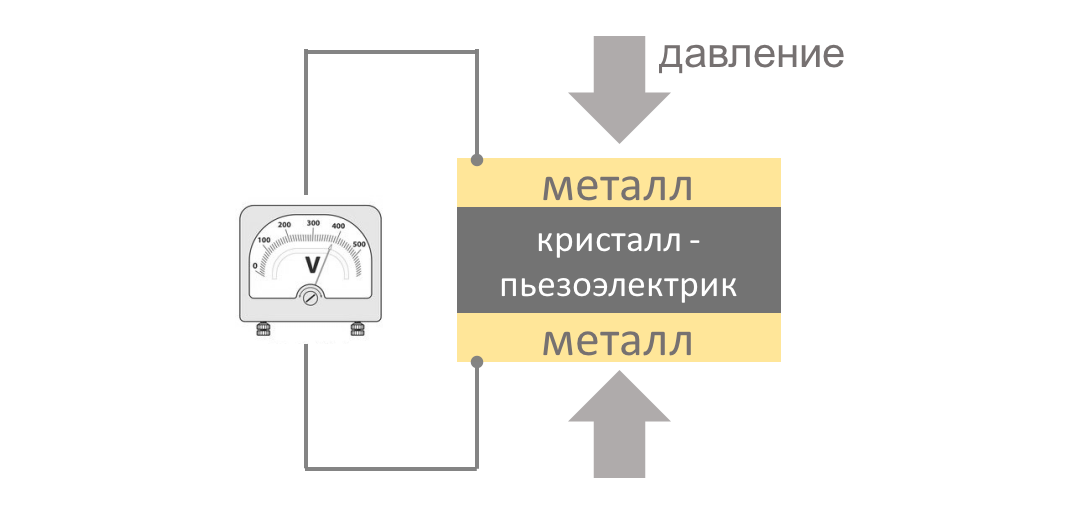
\includegraphics[width=0.4\textwidth]{images/piezo_ther_1.png}}
%   \hfill
%   \subfloat[]{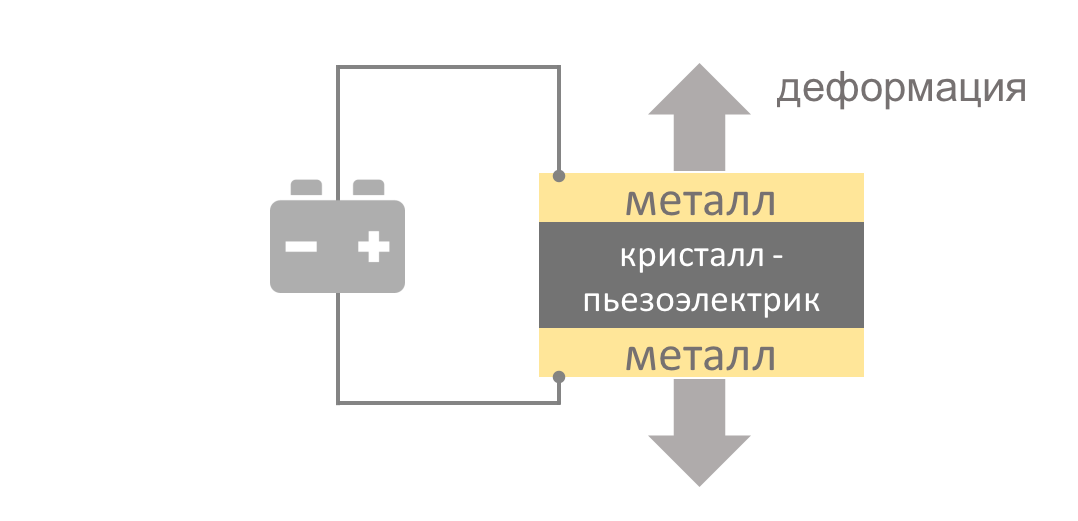
\includegraphics[width=0.45\textwidth]{images/piezo_ther_2.png}}
%   \caption{Свойство пьезоэлектрического кристалла в его простейшем виде для (a)
%    прямого и (b) обратного пьезоэлектрического эффекта}
%   \label{ris:piezo_is}
% \end{figure}

Согласно определению обратного пьезоэлектрического эффекта,
приложенное внешнее электрическое поле $\vec{E}$ является причиной возникновения
в кристаллическом материале деформаций $r_i$. Вектор деформаций пропорционален
величине приложенного напряжения и зависит от пьезоэлектрических свойств материала
в данном направлении. Модуль пьезоэлектрических деформаций $d$ является матрицей,
 с размерностью (3х6) \cite{kedi_1949,Newnham_2005}.

\begin{equation}
  r_j = d_{ij}E_i,
  \label{eq:piezomodule}
\end{equation}
где $i = (1,2,3) = (x,y,z)$, $j = (1,2,3,4,5,6)$, $E_i$ - компонента напряженности электрического поля.

Исходя из уравнения (\ref{eq:piezomodule}) можно судить о том, что поле, приложенное в каком-либо из
направлений, может вызывать деформацию кристалла в любом направлении с коэффициентом пропорциональности $d_{ij}$.
Компоненты деформации  $r_1$, $r_2$ ...$r_6$ можно также обозначать через $x_x$, $y_y$, $z_z$,
$y_z$, $z_x$ и $x_y$ (обозначения Кирхгофа)  \cite{kedi_1949}.

 Например, компонента растяжения/сжатия $r_1= x_x $ соответствует относительному изменения
 длины вдоль данного направления $\frac{\Delta x}{x_0}$ (рис. \ref{ris:deform_piezo}b), а
 компонента сдвиговой деформации соответствует отношению $r_6= x_y = \frac{\Delta x}{y_0}$,
 как показано на рис. \ref{ris:deform_piezo}a.
\begin{figure}[H]
  \centering
  \subfloat[]{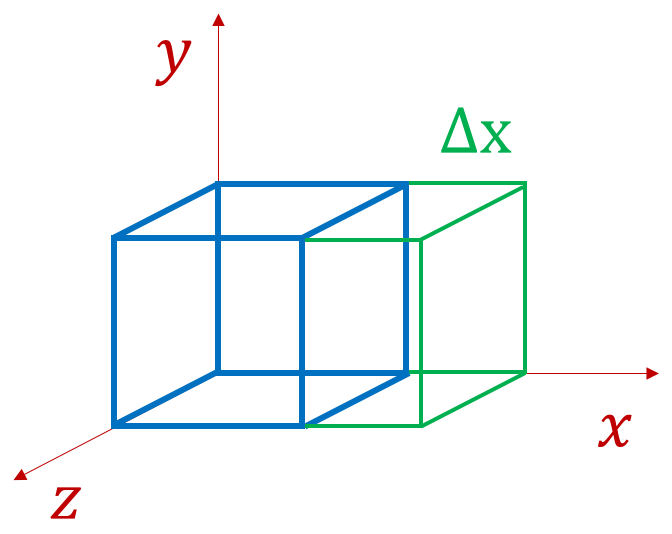
\includegraphics[width=0.45\textwidth]{images/x_x_3d.png}}
  \hfill
  \subfloat[]{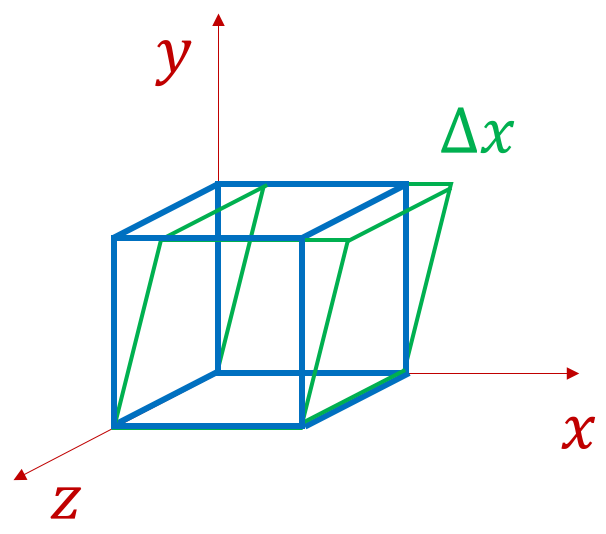
\includegraphics[width=0.45\textwidth]{images/x_y_3d.png}}
  \caption{Схематичное изображение деформации
  растяжения/сжатия $r_1= x_x = \frac{\Delta x}{x_0}$ (a),
   сдвига  $r_6= x_y = \frac{\Delta x}{y_0} $ (b)  }
  \label{ris:deform_piezo}
\end{figure}

Деформации вида $x_y$ и $y_x$ являются связанными и выражаются друг через друга.
На рис. \ref{ris:2x_y_1} представлен пример преобразования сдвиговой деформации
для $x_y = y_x$, такую деформацию описывают только одной компонентой.
С математической точки зрения отождествление $x_y$ с $y_x$
уменьшает число независимых компонент общего тенора деформаций.

\begin{figure}[H]
  \centering
  \subfloat[]{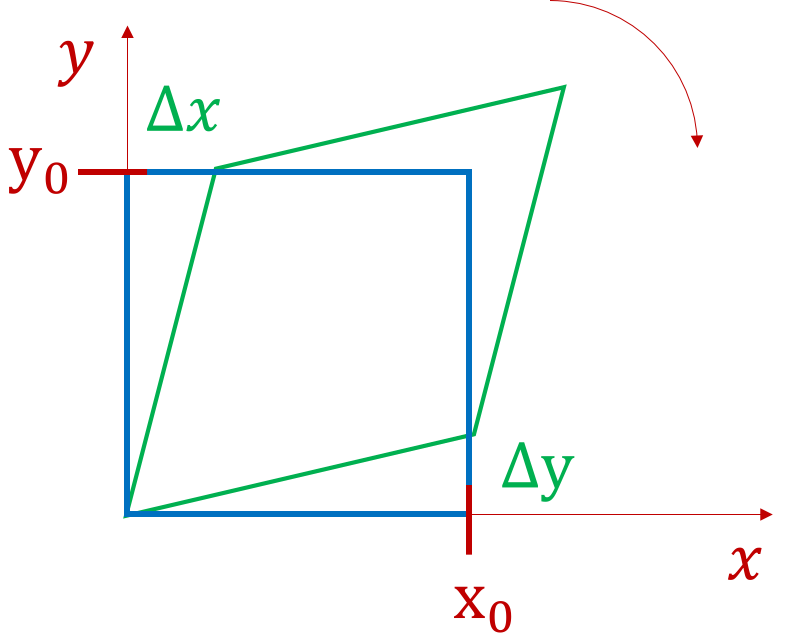
\includegraphics[width=0.45\textwidth]{images/2x_y_1.png}}
  \hfill
  \subfloat[]{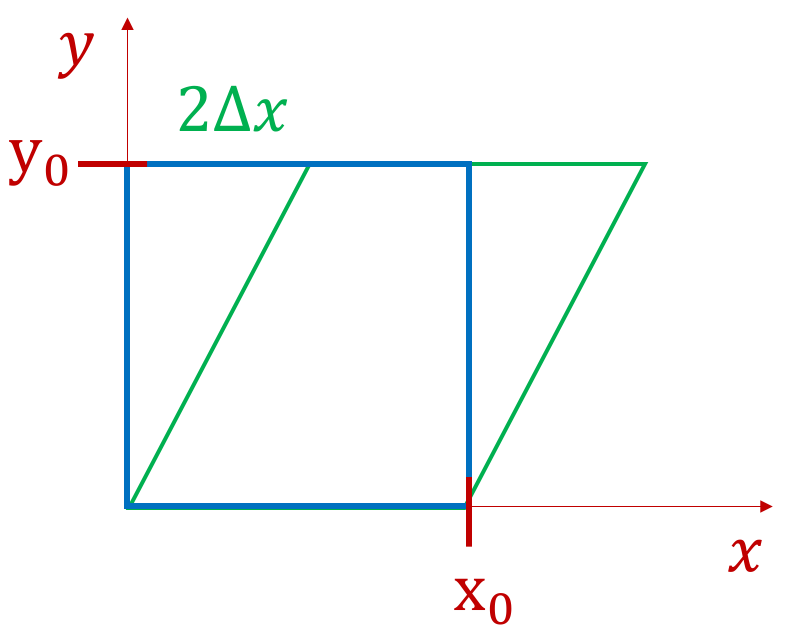
\includegraphics[width=0.45\textwidth]{images/2x_y_2.png}}
  \caption{Переход от двух равных между собой сдвиговых деформации
  $x_y = y_x$ (a) к одной $x_y=\frac{2\Delta x}{y_0}$ (b) с учетом поворота
  поворота образца}
  \label{ris:2x_y_1}
\end{figure}

В развернутой форме выражение (\ref{eq:piezomodule}) выглядит следующим образом:

\begin{equation}
  \begin{pmatrix}
  r_1 \\
  r_2 \\
  r_3 \\
  r_4 \\
  r_5 \\
  r_6
  \end{pmatrix}
   = \begin{pmatrix}
  d_{11} & d_{21}  & d_{31} \\
  d_{12} & d_{22}  & d_{32} \\
  d_{13} & d_{23}  & d_{33} \\
  d_{14} & d_{24}  & d_{34} \\
  d_{15} & d_{25}  & d_{35} \\
  d_{16} & d_{26}  & d_{36}
  \end{pmatrix}
  \begin{pmatrix}
  E_1 \\
  E_2 \\
  E_3
  \end{pmatrix}
  \label{eq:piezomodule_matrica}
\end{equation}

В общем случае все 18 пьезомодулей не зависимы друг от друга. Однако,
под действием операции симметрии кристалл должен полностью совместиться с
самим собой и это касается не только его строения, но и любого физического свойства.
Исходя из принципа Неймана \cite{Shaskolska_1984} физические свойства
 по кристаллографически эквивалентным направлениям должны быть одинаковыми.
Таким образом, пьезоэлектрический эффект может возникнуть только в кристаллах, лишенных центра
симметрии. В 11 из 32 классах точеной группы симметрии нет полярных направлений,
а значит в кристаллах этих классов не может возникать пьезоэффект. Для остальных
классов некоторые пьезомодули могут обратиться в нуль из-за наличия симметрии.
При этом, чем выше симметрия, тем меньше число независимых пьезомодулей.
